
%\text{In order to design a sound level detector, first  
% have to detect the ambient sound}


\justify


Solving electrical circuits is a task that can be reasonably hard. With a higher number of dynamic elements and nodes, the whole calculation process can get chaotic. Having a systematic approach is a critical achievement in getting a viable solution. Even sometimes, computational work can get out of control. That's why we have state-space representation. It enables us to numerically calculate the solution to a system with less computational work. Having represented in inductor voltages, capacitor currents, and their respected derivatives decrease the computational work significantly.
\par 
\bigskip
To summarize the process first, we need to draw the tree of the circuit, including the maximum number of capacitors in its branches, all of the voltage sources, and the least number of inductors. Leftover nodes should be connected to form a tree with resistor branches. Then the capacitor currents can be represented in an equation using fundamental cutsets of their currents, and voltages of inductors can be represented as fundamental loops having only one co-tree branch. These equations form the state space representation
\par
\begin{equation}
\boldmath
\mathbf{\dot{x}=Ax+Bu}
\end{equation}
\par
Here we have ẋ as derivative vector of state variables, A the coefficient matrix, x as state variable vector, B as coefficient matrix and u as input source vector. Here is the process on writing these equations and forming matrices.
\bigskip

\begin{figure}[h]
\centerline{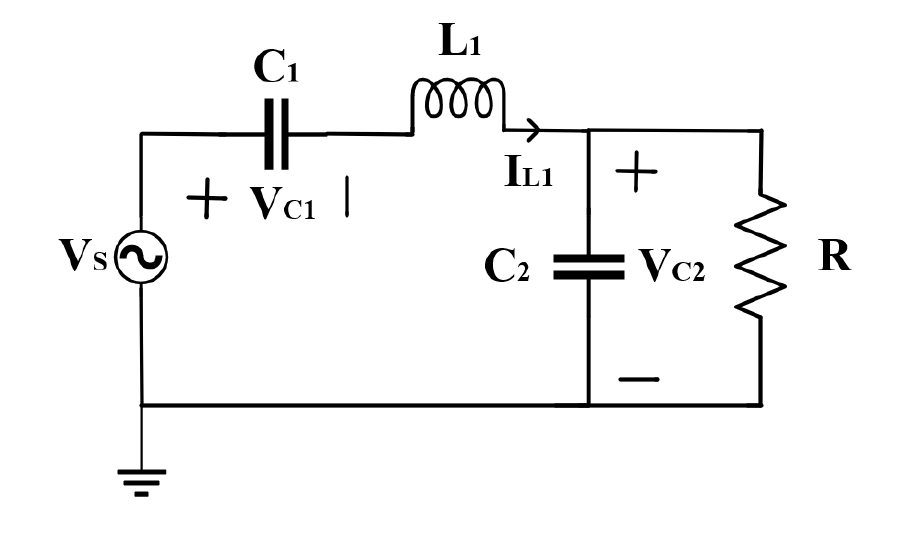
\includegraphics[scale=.35]{Images/circuit.png}}
\caption{Circuit to be solved for \textsubscript{c1}(t),V\textsubscript{c2}(t) and I\textsubscript{L1}(t)}
\label{fig}
\end{figure}

\begin{figure}[h]
\centerline{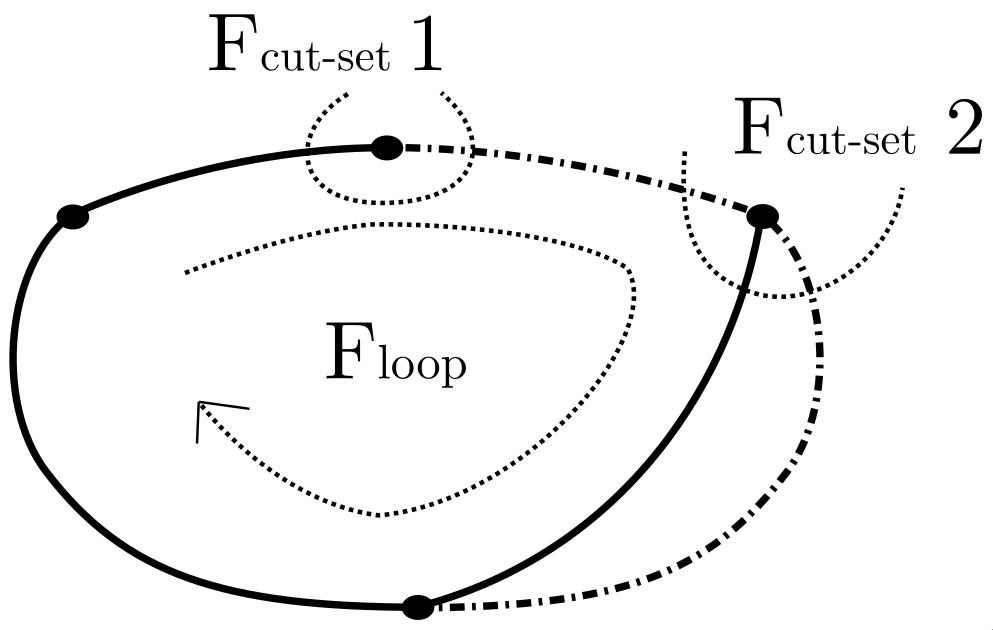
\includegraphics[scale=.25]{Images/graph.png}}
\caption{The graph representation of the circuit with fundamental cut-sets and loop as shown.}
\label{fig}
\end{figure}
\bigskip
\bigskip
\bigskip
\begin{equation}
\text{Node 2 :  }
%\boldmath
\mathrm{I_C_1 = I_L_1}
\end{equation}

\begin{equation}
\text{Node 3  :  }
\mathrm{I_L_1 = I_C_2+V_C_2 / R}
\end{equation}

\begin{equation}
\text{Mesh 1 :  }
\mathrm{V_s + V_C_1 - L_1di/dt -V_C_2 = 0}
\end{equation}
\begin{center} 
\bigskip
If we try to convert this into state-space form;\\
\bigskip
\bigskip
A =
\begin{bmatrix}
0 & 0 & 1/C_1\\
0 & -1/RC_2 & 1/C_2\\
-1/L_1 &-1/L_1&0
\end{bmatrix}
B =
\begin{bmatrix}
0 \\
0 \\
1/L_1
\end{bmatrix}
\end{center} 
\bigskip
Now we can solve this system on MATLAB, using discrete time. What we have is the functions with derivatives as equations in discrete time systems we can add all the infinitesimal values to form the integral of infinitesimal, which is just the variable itself. Matlab script basically does this in a for loop. Main problem with numerically evaluating differential equations is that our time steps should be very small. For my script I take around 2 million samples for a time span. Here is the basic code.



\begin{lstlisting}
clc
clear all
close all
%------------------------------------------------------------
% EE202 Project Part1
% By Ozgur Gulsuna
%Constants---------------------------------------------------
R=100;
L=1/2;
C1=10E-6;
C2=100E-6;

%Resolution in time and time span to be evaluated------------
resolution=20000000;
time_span=2;

%Coefficient Matrices----------------------------------------
A=[0,0,1/C1;0,-1/(R*C2),1/C2;-1/L,-1/L,0];
B=[0;0;1/L];

%Creating a linear time space--------------------------------
time=linspace(0,time_span,resolution);
increment=linspace(1,(resolution),(resolution));

%Empty state Matrix With time dimension----------------------
X=[0;0;0];
X=X*increment;

%Source Vector ----------------------------------------------
U=sin(150*pi*time);

%Main loop that evaluates the integral as a system ----------
for i=increment;
xx= A*X(:,i)+B*U(i);
if i>resolution-1
    break
end
X(:,i+1)=X(:,i)+xx*time_span/resolution;
end

%Plotting the Results----------------------------------------
figure();
subplot(3,1,1);
plot(time,X(1,:));
ylabel("Vc1 (V)");
xlabel("time (t)");
title("Vc1(t)");

subplot(3,1,2);
plot(time,X(2,:));
ylabel("Vc2 (V)");
xlabel("time (t)");
title("Vc2(t)");

subplot(3,1,3);
plot(time,X(3,:));
ylabel("iL1 (A)");
xlabel("time (t)");
title("iL1(t)");

\end{lstlisting}
\begin{center}
Here are the output plots. 
\begin{figure}[h]
\centerline{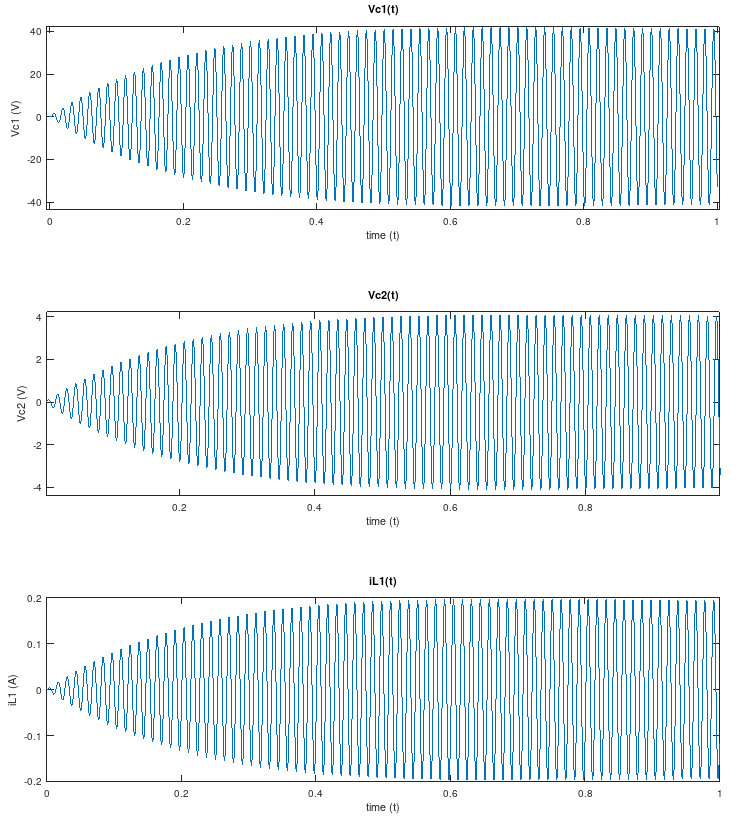
\includegraphics[scale=0.8]{Images/plot-m.png}}
\caption{Voltage of the capacitors and the current of the inductor with respect to time.}
\label{fig}
\end{figure}

\end{center}
